%%%%%%%%%%%%%%%%%%%%%%%%%%%%%%%%%%%%%%%%%
% Short Sectioned Assignment LaTeX Template Version 1.0 (5/5/12)
% This template has been downloaded from: http://www.LaTeXTemplates.com
% Original author:  Frits Wenneker (http://www.howtotex.com)
% License: CC BY-NC-SA 3.0 (http://creativecommons.org/licenses/by-nc-sa/3.0/)
%%%%%%%%%%%%%%%%%%%%%%%%%%%%%%%%%%%%%%%%%

%----------------------------------------------------------------------------------------
%	PACKAGES AND OTHER DOCUMENT CONFIGURATIONS
%----------------------------------------------------------------------------------------

\documentclass[paper=a4, fontsize=11pt]{scrartcl} % A4 paper and 11pt font size

% ---- Entrada y salida de texto -----

\usepackage[T1]{fontenc} % Use 8-bit encoding that has 256 glyphs
\usepackage[utf8]{inputenc}
\usepackage{fourier} % Use the Adobe Utopia font for the document - comment this line to return to the LaTeX default

% ---- Idioma --------

\usepackage[spanish, es-tabla]{babel} % Selecciona el español para palabras introducidas automáticamente, p.ej. "septiembre" en la fecha y especifica que se use la palabra Tabla en vez de Cuadro

% ---- Otros paquetes ----

\usepackage{url} % ,href} %para incluir URLs e hipervínculos dentro del texto (aunque hay que instalar href)
\usepackage{amsmath,amsfonts,amsthm} % Math packages
%\usepackage{graphics,graphicx, floatrow} %para incluir imágenes y notas en las imágenes
\usepackage{graphics,graphicx, float} %para incluir imágenes y colocarlas
\usepackage{epstopdf}
\usepackage[gen]{eurosym} %para incluir el símbolo del euro
\usepackage{cite} %para incluir citas del archivo <nombre>.bib
%\graphicspath{/images}

% Para hacer tablas comlejas
%\usepackage{multirow}
%\usepackage{threeparttable}

%\usepackage{sectsty} % Allows customizing section commands
%\allsectionsfont{\centering \normalfont\scshape} % Make all sections centered, the default font and small caps

\usepackage{fancyhdr} % Custom headers and footers
\pagestyle{fancyplain} % Makes all pages in the document conform to the custom headers and footers
\fancyhead{} % No page header - if you want one, create it in the same way as the footers below
\fancyfoot[L]{} % Empty left footer
\fancyfoot[C]{} % Empty center footer
\fancyfoot[R]{\thepage} % Page numbering for right footer
\renewcommand{\headrulewidth}{0pt} % Remove header underlines
\renewcommand{\footrulewidth}{0pt} % Remove footer underlines
\setlength{\headheight}{13.6pt} % Customize the height of the header

\numberwithin{equation}{section} % Number equations within sections (i.e. 1.1, 1.2, 2.1, 2.2 instead of 1, 2, 3, 4)
\numberwithin{figure}{section} % Number figures within sections (i.e. 1.1, 1.2, 2.1, 2.2 instead of 1, 2, 3, 4)
\numberwithin{table}{section} % Number tables within sections (i.e. 1.1, 1.2, 2.1, 2.2 instead of 1, 2, 3, 4)

\setlength\parindent{0pt} % Removes all indentation from paragraphs - comment this line for an assignment with lots of text

\newcommand{\horrule}[1]{\rule{\linewidth}{#1}} % Create horizontal rule command with 1 argument of height


%----------------------------------------------------------------------------------------
%	TÍTULO Y DATOS DEL ALUMNO
%----------------------------------------------------------------------------------------

\title{
\normalfont \normalsize
\textsc{\textbf{Ingeniería de Servidores (2016-2017)} \\ Grado en Ingeniería Informática \\ Universidad de Granada} \\ [25pt] % Your university, school and/or department name(s)
\horrule{0.5pt} \\[0.4cm] % Thin top horizontal rule
\huge Memoria Práctica 3 \\ % The assignment title
\horrule{2pt} \\[0.5cm] % Thick bottom horizontal rule
}

\author{Adrián Morente Gabaldón} % Nombre y apellidos

\date{\normalsize\today} % Incluye la fecha actual

%----------------------------------------------------------------------------------------
% DOCUMENTO
%----------------------------------------------------------------------------------------

\begin{document}

\maketitle % Muestra el Título

\newpage %inserta un salto de página

\tableofcontents % para generar el índice de contenidos

\listoffigures

\listoftables

\newpage


\section{a) ¿Qué archivo le permite ver qué programas se han instalado con el gestor de paquetes? b) ¿Qué significan las terminaciones \emph{1.gz} o \emph{2.gz} de los archivos en ese directorio?}

	\subsection{Consulta de los paquetes instalados con APT}
	Como comentamos siempre en clase de prácticas, una de las cosas que tenemos que revisar como administradores de sistemas son los archivos \emph{.log}, los cuales contienen frecuentemente información relevante sobre paquetes instalados o servicios ofrecidos. En este caso, podemos consultar los paquetes instalados de APT a través del archivo ubicado en \emph{/var/log/apt/history.log}. En la misma carpeta podemos encontrar también el archivo \emph{term.log}, que contiene los resultados de instalación, consulta y borrado de paquetes realizados por APT. \\
	En la siguiente imagen, vemos el contenido del directorio mencionado, e imprimimos el contenido del fichero \emph{history.log} incluido en tal sitio; ya que en él encontramos la información pedida por el enunciado:
	\begin{figure}[H]
		\centering
		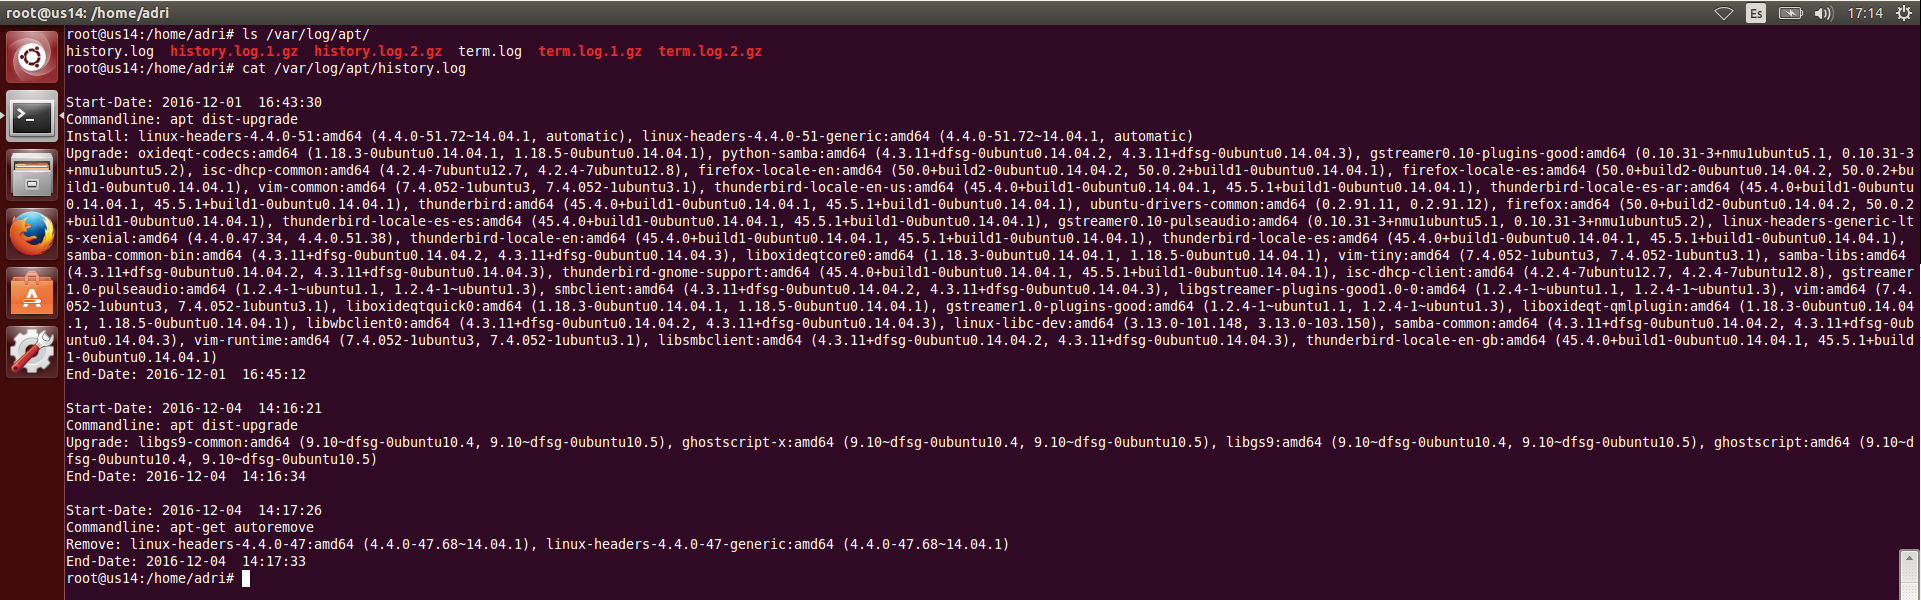
\includegraphics[scale=0.3]{apt-history}
		\caption{Consulta de los paquetes instalados con APT en el directorio /var/log/apt. - Adrián Morente Gabaldón [04/12/2016]}
		\label{figura1}
	\end{figure}
	En cuanto a la extensión del contenido del archivo, que vemos que es muy reducida, hablaremos de ello en el siguiente apartado del ejercicio. En este caso, podemos ver en los apartados \textbf{Commandline: apt ...} que las últimas acciones que realicé en la administración de Ubuntu Server fueron las actualizaciones del sistema, con los consiguientes borrados automáticos de programas y/o paquetes innecesarios. \\
	A continuación, vemos parte del contenido del archivo \emph{term.log}, que concuerda con las actualizaciones y borrados realizados arriba, ya que aquí se recogen los resultados de dichas acciones:
	\begin{figure}[H]
		\centering
		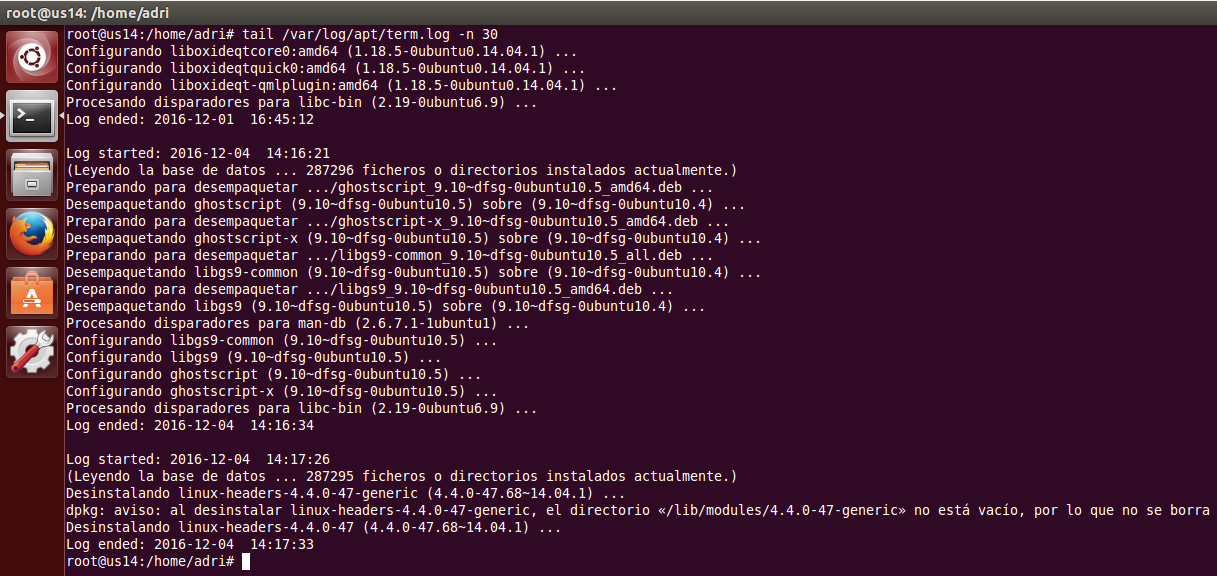
\includegraphics[scale=0.4]{apt-term}
		\caption{Contenido del archivo \emph{term.log} y los resultados de la ejecución de APT. - Adrián Morente Gabaldón [04/12/2016]}
		\label{figura2}
	\end{figure}

	\subsection{Archivos \emph{1.gz} y \emph{2.gz} del gestor APT}
	Como podemos ver en los manuales oficiales de GNU \cite{gzip}, los archivos con extensión \emph{.gz} son archivos comprimidos manejados por sistemas operativos basados en Unix. El gestor de paquetes APT deposita el historial y los resultados de sus ejecuciones en los archivos \emph{history.log} y \emph{term.log} respectivamente, como hemos visto antes; pero conforme esos archivos comienzan a tener un tamaño elevado, el sistema decide comprimir su contenido para ahorrar espacio. Por ejemplo, para el archivo \emph{history.log}, comprimirá todo su contenido en un nuevo archivo \emph{history.log.X.gz} siendo X el número de veces que se ha realizado esta acción. Es decir, si el sistema ha hecho esto tres veces, tendremos los tres archivos \emph{history.log.1.gz}, \emph{history.log.2.gz} y \emph{history.log.3.gz}; siendo siempre más reciente aquel con numeración menor.

\section{¿Qué archivo ha de modificar para programar una tarea? Escriba la línea necesaria para ejecutar una vez al día una copia del directorio ~/codigo a ~/seguridad/\$fecha donde \$ fecha es la fecha actual (puede usar el comando date).}
Para informarnos sobre el uso de \emph{cron} (herramienta ya utilizada en la asignatura de Sistemas Operativos) podemos utilizar el manual a través de la línea de comandos, aunque en mi caso utilizaré también la documentación oficial de Oracle al respecto \cite{cron}, que en mi caso es más ilustrativa para el uso de dicha herramienta. \\
Como vemos en la web, el archivo modificado al programar una tarea es \textbf{/var/spool/cron/crontabs}, pero es preferible no modificarlo directamente; sino hacerlo a través de la ejecución de la herramienta \emph{crontab}, como haremos en este caso práctico.
Para empezar, crearemos el script \emph{script\_seguridad.sh} que después ejecutaremos periódicamente, que tendrá el siguiente contenido:
\begin{verbatim}
	#!/bin/bash
	  #guarda la fecha actual en la variable
	date=$(date '+%Y%m%d_%H%M%S')
	  #si no existe, crea el directorio (primera vez)
	mkdir -p /seguridad/$date_time
	  #copia los archivos de /codigo a /seguridad/fecha
	cp -r ~/codigo/* ~/seguridad/$date_time
\end{verbatim}
A continuación, daremos permiso de ejecución al script (\emph{chmod u+x script\_seguridad.sh}) y crearemos varios ficheros de texto plano en el directorio \emph{~/codigo} con el contenido de prueba que queramos. \\
Antes de programar el archivo, volvamos a mirar la documentación de Oracle para ``refrescar la memoria'' en cuanto a la sintaxis de éstos \cite{cron-sintaxis}; y veremos que el orden de sus parámetros es:
\begin{verbatim}
<minuto> <hora> <día_mes> <mes> <día_semana> <comandos>
\end{verbatim}
Para terminar, crearemos el archivo \emph{cron} pero tal y como hemos dicho antes: sin acceder al fichero directamente sino a través de la herramienta \emph{crontab}. Como queremos que se ejecute una vez al día, podemos fijar que sus parámetros de ejecución sean siempre a las 5 de la tarde, lo cual sería de la siguiente forma:
\begin{lstlisting}[language=bash]
	crontab -e {0 17 * * * ~./script_seguridad.sh}
\end{lstlisting}

\section{Pruebe a ejecutar el comando, conectar un dispositivo USB y vuelva a ejecutar el comando. Copie y pegue la salida del comando. (considere usar dmesg | tail). Comente qué observa en la información mostrada.}
Como sabemos, el comando \emph{dmesg} puede ser muy útil para detectar problemas o cambios en el hardware conectado al kernel de un sistema; su uso es sencillo y da pie a muchas opciones (apenas usadas), según vemos en el manual del proyecto \emph{Linux Information Project} \cite{dmesg}. \\
Pasemos a ejecutar el comando \emph{dmesg | tail} para mostrar parte de esta información, y procedemos a insertar un pendrive USB en el ordenador, que seleccionamos a través del menú ``Dispositivos'' de la máquina virtual en VirtualBox de forma que el sistema virtual lo reconozca. Hecho esto, nos encontraremos con la siguiente imagen, en la que podemos ver cómo el kernel pasa a detectar el pendrive insertado, dándonos información del tipo de dispositivo (\emph{USB DISK 2.0}), el tamaño total (16GiB, 14.9GiB utilizables, en mi caso), el tamaño de cada bloque de datos en bytes (512B), y el modo de protección de escritura de datos (desactivado, ahora mismo) entre otros.
\begin{figure}[H]
	\centering
	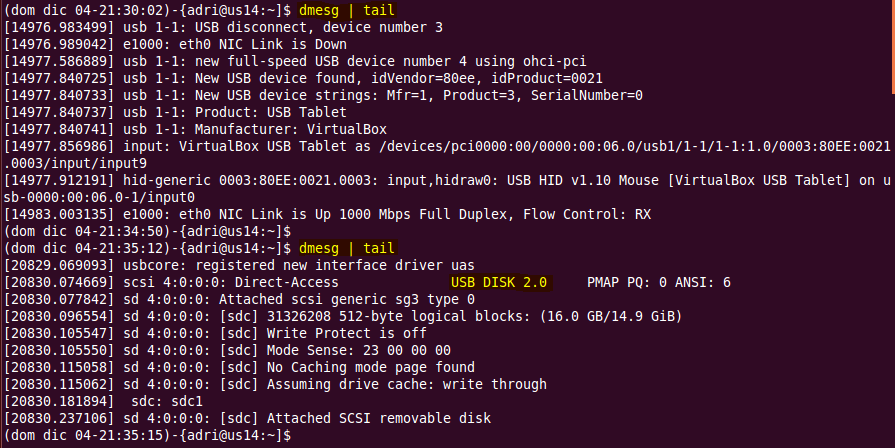
\includegraphics[scale=0.5]{dmesg}
	\caption{Muestra de los resultados recopilados del kernel por \emph{dmesg}. - Adrián Morente Gabaldón [04/12/2016]}
	\label{figura3}
\end{figure}

\section{Ejecute el monitor de ``System performance'' y muestre el resultado. Incluya capturas de pantalla comentando la información que aparece.}

\section{Cree un recopilador de datos definido por el usuario (modo avanzado) que incluya tanto el contador de rendimiento como los datos de seguimiento: 1) Todos los referentes al procesador, al proceso y al servicio web. 2) Intervalo de muestra 15 segundos. 3) Almacene el resultado en el directorio Escritorio/logs. 4) Incluya las capturas de pantalla de cada paso.}

\section{Visite la web del proyecto y acceda a la demo que proporcionan (http://demo.munin-monitoring.org/) donde se muestra cómo monitorizan un servidor. Monitorice varios parámetros y haga capturas de pantalla de lo que está mostrando comentando qué observa.}

\section{Escriba un breve resumen sobre alguno de los artículos donde se muestra el uso de strace o busque otro y coméntelo.}
En mi caso, haré un análisis del segundo artículo ofrecido en la práctica, proveniente del blog oficial de \textbf{SoftLayer, una compañía de IBM} \cite{softlayer-strace}. \\
Para empezar, plantean una descripción que nos sitúa en el marco de uso de la herramienta \emph{strace}, haciéndonos ver que su utilización va orientada a los administradores de sistemas (en este caso, nosotros); y que a través de su ejecución podemos analizar y corregir los errores de los servicios que ofrecemos mostrándonos las llamadas al sistema y las señales resultantes de la ejecución de dichos servicios. Gracias a esto, a través de los archivos \emph{.log} podemos ver cuál de los parámetros no están bien configurados o qué paquetes están fallando de alguna forma. \\


descartar que sea una herramienta para programadores, ya que está destinada a los administradores de sistemas (en este caso, nosotros); dado que su utilización va orientada a la detección y solución de errores en la ejecución de los servicios que ofrecemos en nuestro sistema. Para poder mostrarnos cuál de nuestros programas está fallando, o qué está realizando cada uno de ellos, esta herramienta nos muestra las llamadas y las señales del sistema resultantes de dichos programas.

\section{Escriba un script en Python o PHP y analice su comportamiento usando el profiler presentado.}

\section{Acceda a la consola MySQL (o a través de phpMyAdmin) y muestre el resultado de mostrar el ``profile'' de una consulta (la creación de la BD y la consulta la puede hacer libremente).}


\bibliography{citas}
\bibliographystyle{plain}
\end{document}
